\documentclass{article}
\usepackage{graphicx}
\usepackage{wrapfig}
\usepackage{amsmath}
\usepackage{subcaption}
\title{CuO Analysis Details}
\author{Shivesh Pathak}
\begin{document}
\maketitle
\section{Experiment}
APES measurements in 1996 indicate that the low-lying states of the CuO molecule are composed of 3d$^9$ and 3d$^10$ states, namely 9 and 10 electrons on the copper d orbitals [ref 48.pdf].

\begin{wrapfigure}{r}{0.4\textwidth}
  \begin{center}
    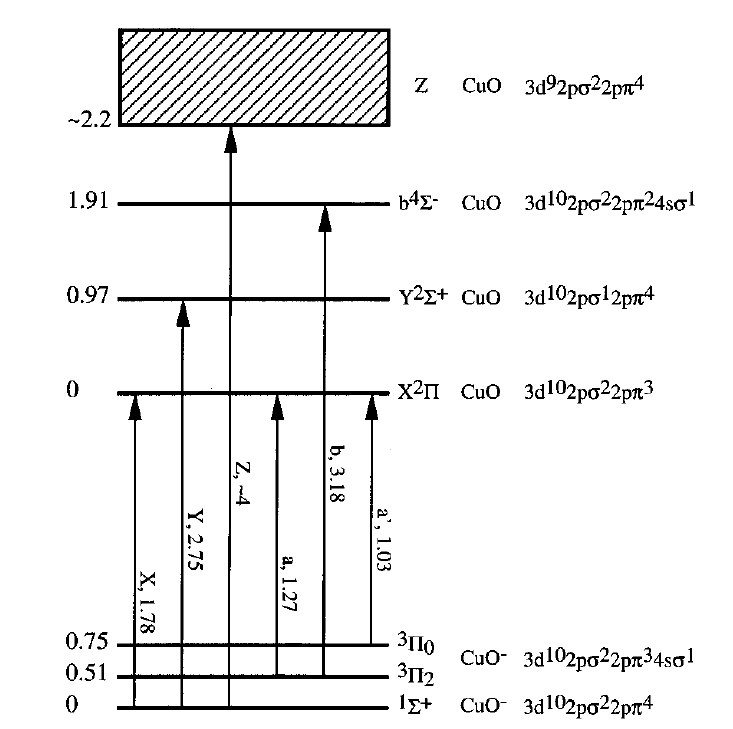
\includegraphics[width=0.3\textwidth]{APES.png}
  \end{center}
  \caption{APES measurements on CuO molecule.}
\end{wrapfigure}

They find the ground state to be of type $X^2\Pi$ and the first excited state to be of type $Y^2\Sigma^+$, which are consistent with higher resolution PES measurements and various other theoretical and experimental measurements [ref, \textbf{clean this up}]. The $X^2\Pi \rightarrow Y^2\Sigma^+$ excitation corresponds to an excitation $O p_\sigma \rightarrow O p_\pi$, and has a measured energy of 0.97 eV. The PES measurements also find a block of excitations starting at 2.20 eV which correspond to the 3d$^9$ excited states of CuO. Earlier measurements have found similar results. Both these PES measurements and Laser Induced Flourescence measurements in 1980 [ref] have found a quartet state at 1.91 eV. This state has been assigned as $^4\Sigma$ state, but the argumentation for its assignment is quite loose and based on a simple single particle model. Shown below are the most recent APES measurements for the CuO molecule, all state assignments except for the $b$ state have been verified by other experiments.

Given that the lowest energy states are 3d10 in character and higher energy excited states at 3d9, it is informative to look at the properties of the copper atom with 10 and 9 electrons respectively. The Cu$^+$ atom can have either configurations 3d$^10$4s$^0 (^1S)$ or 3d$^9$4s$^1 (^3D, ^1D)$ [ref]. The $^3D$ is lower in energy than the $^1D$ state by about 0.54 eV, indicating that a Hund's coupling between the Cu 4s and 3d orbitals of $J_H = -0.54 eV$. 

\section{Sampling scheme}
In order to do DMD we need to densely sample the low energy space. In our case here, we will define the LES as the span of some base states. Since we know that our system has a low energy $3d9$ and $3d10$ sector, we will consider base states with either 9 or 10 electrons in the d-orbitals. Further, in order to consider the effects of a possible Hund's coupling arising in our effective theory from the Cu $J_H$, we will need to consider states with both $S_z=1/2, 3/2$. When moving to QMC, we will not be able to consider linear combinations of states with different $S_z$, so in order to sample the effect of $J_H$ densely, we would also like to consider "spin-flip partner" states in the $S_z=1/2$ sector. Consider for example a state 3d$^9$2p$_{pi}^3$4s$^1$ in the $S_z=1/2$ sector. The half-filled orbitals can have electrons with configuration $up\ up\ dn$ or $up\ dn\ up$, the prior which would have a Hund's energy $\frac{1}{2}J_H$ and the latter $-\frac{1}{2}J_H$. We would also like to work with single determinant base states, since we have found that single determinant Slater-Jastrow wave functions are quite accurate for transition metal oxide molecules [ref]. In order to meet all of these considerations, we chose to collect base states by using spin and spatial-symmetry targeted unrestricted Kohn Sham eigenstates. We generated all unique base states in the 3d9 and 3d10 sectors using this method. In order to sample the span of the base states, namely our defined LES, we used a shell sampling technique which samples in shells of fixed radius around each of the base states using base state weights of 0.1 - 1.0 in increments of 0.1. Our final set of states in our span were then multiplied by a three-body Jastrow factor, which was optimized on the UKS ground state, and passed into DMC with a timestep of 0.01 and Tmoves on to calculate the 1-/2-rdms and total energy.

\section{RDM basis}
There were two choices of the RDM basis that we could have used, either an IAO basis or an MO basis. The IAO basis is more theoretically pleasing because it's a set of functions which best capture the variation between the the Cu 3d, O 2p, and Cu 4s orbitals from our different base states. However, the IAO basis has the drawback that many parameters will be correlated, for example $n_{p_\pi}$ and $t_\pi$. The MO basis choice is more arbitrary because we simply chose a set of spatially symmetric ($p_x, p_y$ look identical for example) ROKS molecular orbitals, since we don't know a way of constructing "intrinsic molecular orbitals." The MOs however yield the benefit that they are decorrelated for the most part, because to zeroth order the excitations of CuO look very similar to single-particle molecular orbital excitations. I therefore chose to do my model analysis using a mixture of both bases, namely using an MO basis for the non-interacting parts (n, t) but using an IAO basis for the interacting pieces (J, U, etc.).

\section{Model selection}
Model selection required both an understanding of the CuO molecule's low energy excitations and some statistical analysis. We know that the lowest energy excitations of CuO are between the O p and Cu 4s orbitals, as these are the only excitations which allow for a 3d10 configuration. Further, given that we will be including 3d9 states, it's clear that we will need at least consider the following non-interacting parameters:
$$\bar{\epsilon}_d, \bar{\epsilon}_z, \bar{\epsilon}_\pi, \bar{\epsilon}_s, \bar{t}_\pi, \bar{t}_{d_z^2 z}, \bar{t}_{4s z}, \bar{t}_{dz^2 4s}$$

Here the bars indicate parameters corresponding to RDM elements evaluated on our MO basis. In addition to these parameters, we know that the Cu$^+$ atom has a Hund's coupling, so we will consider a parameter $J_{sd}$ which is Hund's coupling between the Cu 4s and Cu 3d orbitals. Finally, some of our base states have a $4s^2$ occupation, and therefore including a $U_{4s}$ is necessary. Our final proposed model then looks like: 

$$ \boxed{\text{Proposed model: }\bar{\epsilon}_d, \bar{\epsilon}_z, \bar{\epsilon}_\pi, \bar{\epsilon}_s, \bar{t}_\pi, \bar{t}_{d_z^2 z}, \bar{t}_{4s z}, \bar{t}_{dz^2 4s}, J_{sd}, U_{4s}}$$

Since we know that $\bar{\epsilon}_d + \bar{\epsilon}_z + \bar{\epsilon}_\pi + \bar{\epsilon}_s = $ Const, we can eliminate $\bar{\epsilon}_d$ from our model since it is linearly dependent on the rest of the parameters. The left over occupation energies are certainly required in our model, given the knowledge we have of our low energy space. Since we know that $U_{4s}$ is required to describe the $4s^2$ states and that the $J_{sd}$ will probably play an important role as well, we just need to do model selection on the four hopping parameters. Below are 5-fold CV linear regressions using \textit{every} model which includes the $\bar{\epsilon}, J_{sd}, U_{4s}$ parameters above and one element in the power set of $\bar{t}_\pi, \bar{t}_{d_z^2 z}, \bar{t}_{4s z}, \bar{t}_{dz^2 4s}$. 

\begin{figure}
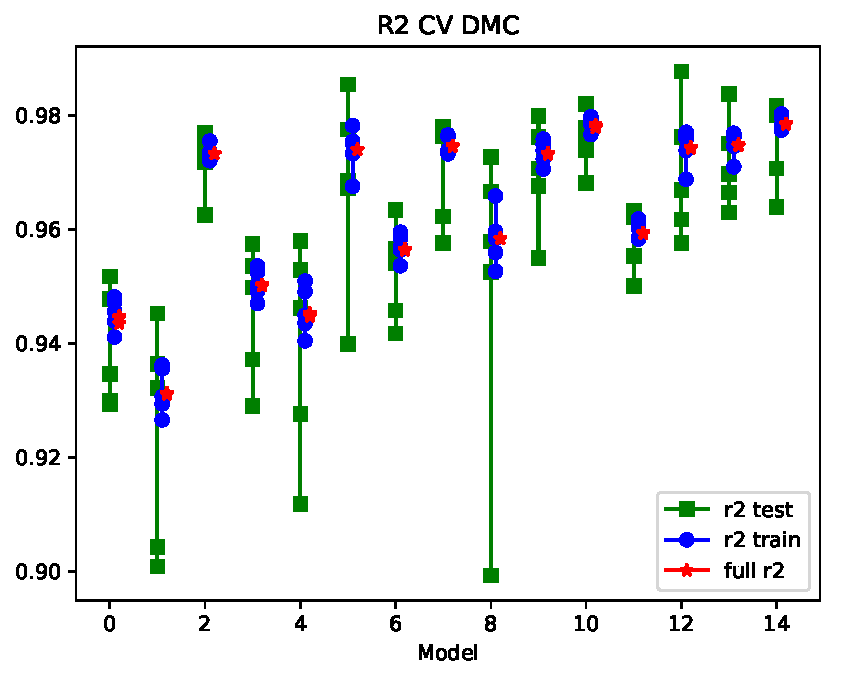
\includegraphics[width=1.0\textwidth]{../qwalk/ub3lyp_s1_/analysis/cv_valid.pdf}
\caption{5-fold CV regressions for model selection}
\end{figure}

The models are increasing in complexity from left-to-right, and it's clear that the fourth model listed here is as accurate as the most complex model, and significantly simpler. Therefore, we selected that model as it captures the most variation with the fewest parameters. The selected model then looks like this: 
$$ \boxed{\text{Selected model: }\bar{\epsilon}_z, \bar{\epsilon}_\pi, \bar{\epsilon}_s, \bar{t}_\pi, J_{sd}, U_{4s}}$$

\section{Model fitting}
We conducted a weighted least squares on our samples in order to fit the six parameters in our selected model. The higher density of states with $3d9$ occupation made it so that an unweighted linear regression would fit in a biased way towards the $3d9$ states, leaving the $3d10$ states fit very poorly. The weighting function we used was $e^{-\beta E_{DMC}}$, where $\beta$ is a variable "temperature" which was varied from 0.25 to 3.75 in increments of 0.25. We find that in the range of $\beta \in {1.5, 2.5}$ the model does not change very much, therefore we select a model at $\beta = 2.0$, which leads to the following set of regressed parameters:
\begin{multline}
 \boxed{\text{Final model }  (\beta=2): \bar{\epsilon}_z = 1.06(6) eV, \bar{\epsilon}_\pi = 2.12(5) eV, \bar{\epsilon}_s = 3.08(4) eV}\\
\boxed{\bar{t}_\pi = 0.52(4) eV, J_{sd} = -0.5(1) eV, U_{4s} = 3.9(2) eV}
\end{multline}

In order to look at the predictions of this model, we can rotate the MO basis elements into the IAO basis elements. Doing so yields the following more complicated model (note the lack of bars on the model parameters now!):

\begin{multline}
 \boxed{\text{Final model }  (\beta=2): \epsilon_{d_\delta} = 0.00 eV, \epsilon_{d_\pi} = -0.10 eV, \epsilon_{d_z^2} = 0.41 eV }\\
 \boxed{\epsilon_z = 1.2 eV, \epsilon_\pi = 2.21 eV, \epsilon_s = 2.44 eV}\\
\boxed{t_\pi = -0.22 eV, t_{d_z^2 s} = 0.38 eV, t_{s z} = 0.80 eV, t_{d_z^2 z} = 0.70 eV}\\
\boxed{ , J_{sd} = -0.5(1) eV, U_{4s} = 3.9(2) eV}
\end{multline}

\section{Comparison to DFT model}
We can then do an exact diagonalization on this model Hamiltonian, which was accomplished using an FCI solver for a custom Hamiltonian in PySCF [ref]. Show in the figures below are the lowest lying eigenstates of this model Hamiltonian for the full range of $\beta$, showing the energies and occupations of different orbitals. We can see that as we let $2.5 > \beta > 1.25 $ the model is fairly stable. The ground state of our model matches that of experiment, namely it has an electron configuration of $Cu 3d^{10} O 2p_z^{1.75} O 2p_\pi^3 Cu 4s^{0.4}$, which would map to the approximate nominal filling of $Cu 3d^{10} O 2p_z^{2} O 2p_\pi^3 Cu 4s^{0}.$ This is also an $S_z=1/2$ state as expected in experiment. The first excited state in this range of $\beta$s is another $S_z=1/2$ state with occupations $Cu 3d^{9.7} O 2p_z^{1.2} O 2p_\pi^4 Cu 4s^{0.3}$, which would map to the approximate nominal filling of $Cu 3d^{10} O 2p_z^{1} O 2p_\pi^4 Cu 4s^{0}.$ This state is at an energy of 1 eV which matches the APES measurements up to a tenth of an eV! The first $3d^9$ state is at around 2.2 eV, which again matches the predictions of the APES measurements. Aside from these states, there are also various states with $S_z=3/2$ which our model predicts to be low in energy. For example, there is an $S_z=3/2$ state with occupation at around 1.4 eV with occupations $Cu 3d^{9.7} O 2p_z^{2.0} O 2p_\pi^2 Cu 4s^{1.0}$, which would map to the approximate nominal filling of $Cu 3d^{10} O 2p_z^{2} O 2p_\pi^2 Cu 4s^{1}.$ As predicted from the anion case, the lowest $S_z=3/2$ state is indeed a $O p_\pi \rightarrow Cu 4s$ excitation. There if another state at 2.0 eV which is $S_z =3/2$ and which corresponds to an $O p_z \rightarrow Cu 4s$ state. Therefore our model predicts that the measured state in APES is indeed a quartet state, however it should have $\Pi$ symmetry. The $\Sigma$ symmetry quartet state, which is indeed the lowest energy $S_z=3/2$ state, resides at an energy very close to the $^2Y$ state and may not have been able to resolve. Overall, our model matches every experimentally measured and rigorously confirmed eigenstate of CuO. We further argue that the labeling of a state at 2.0 eV as $^4\Sigma$ is faulty and it should be $^4\Pi$.

\begin{figure}
\centering
\begin{subfigure}{.5\textwidth}
  \centering
  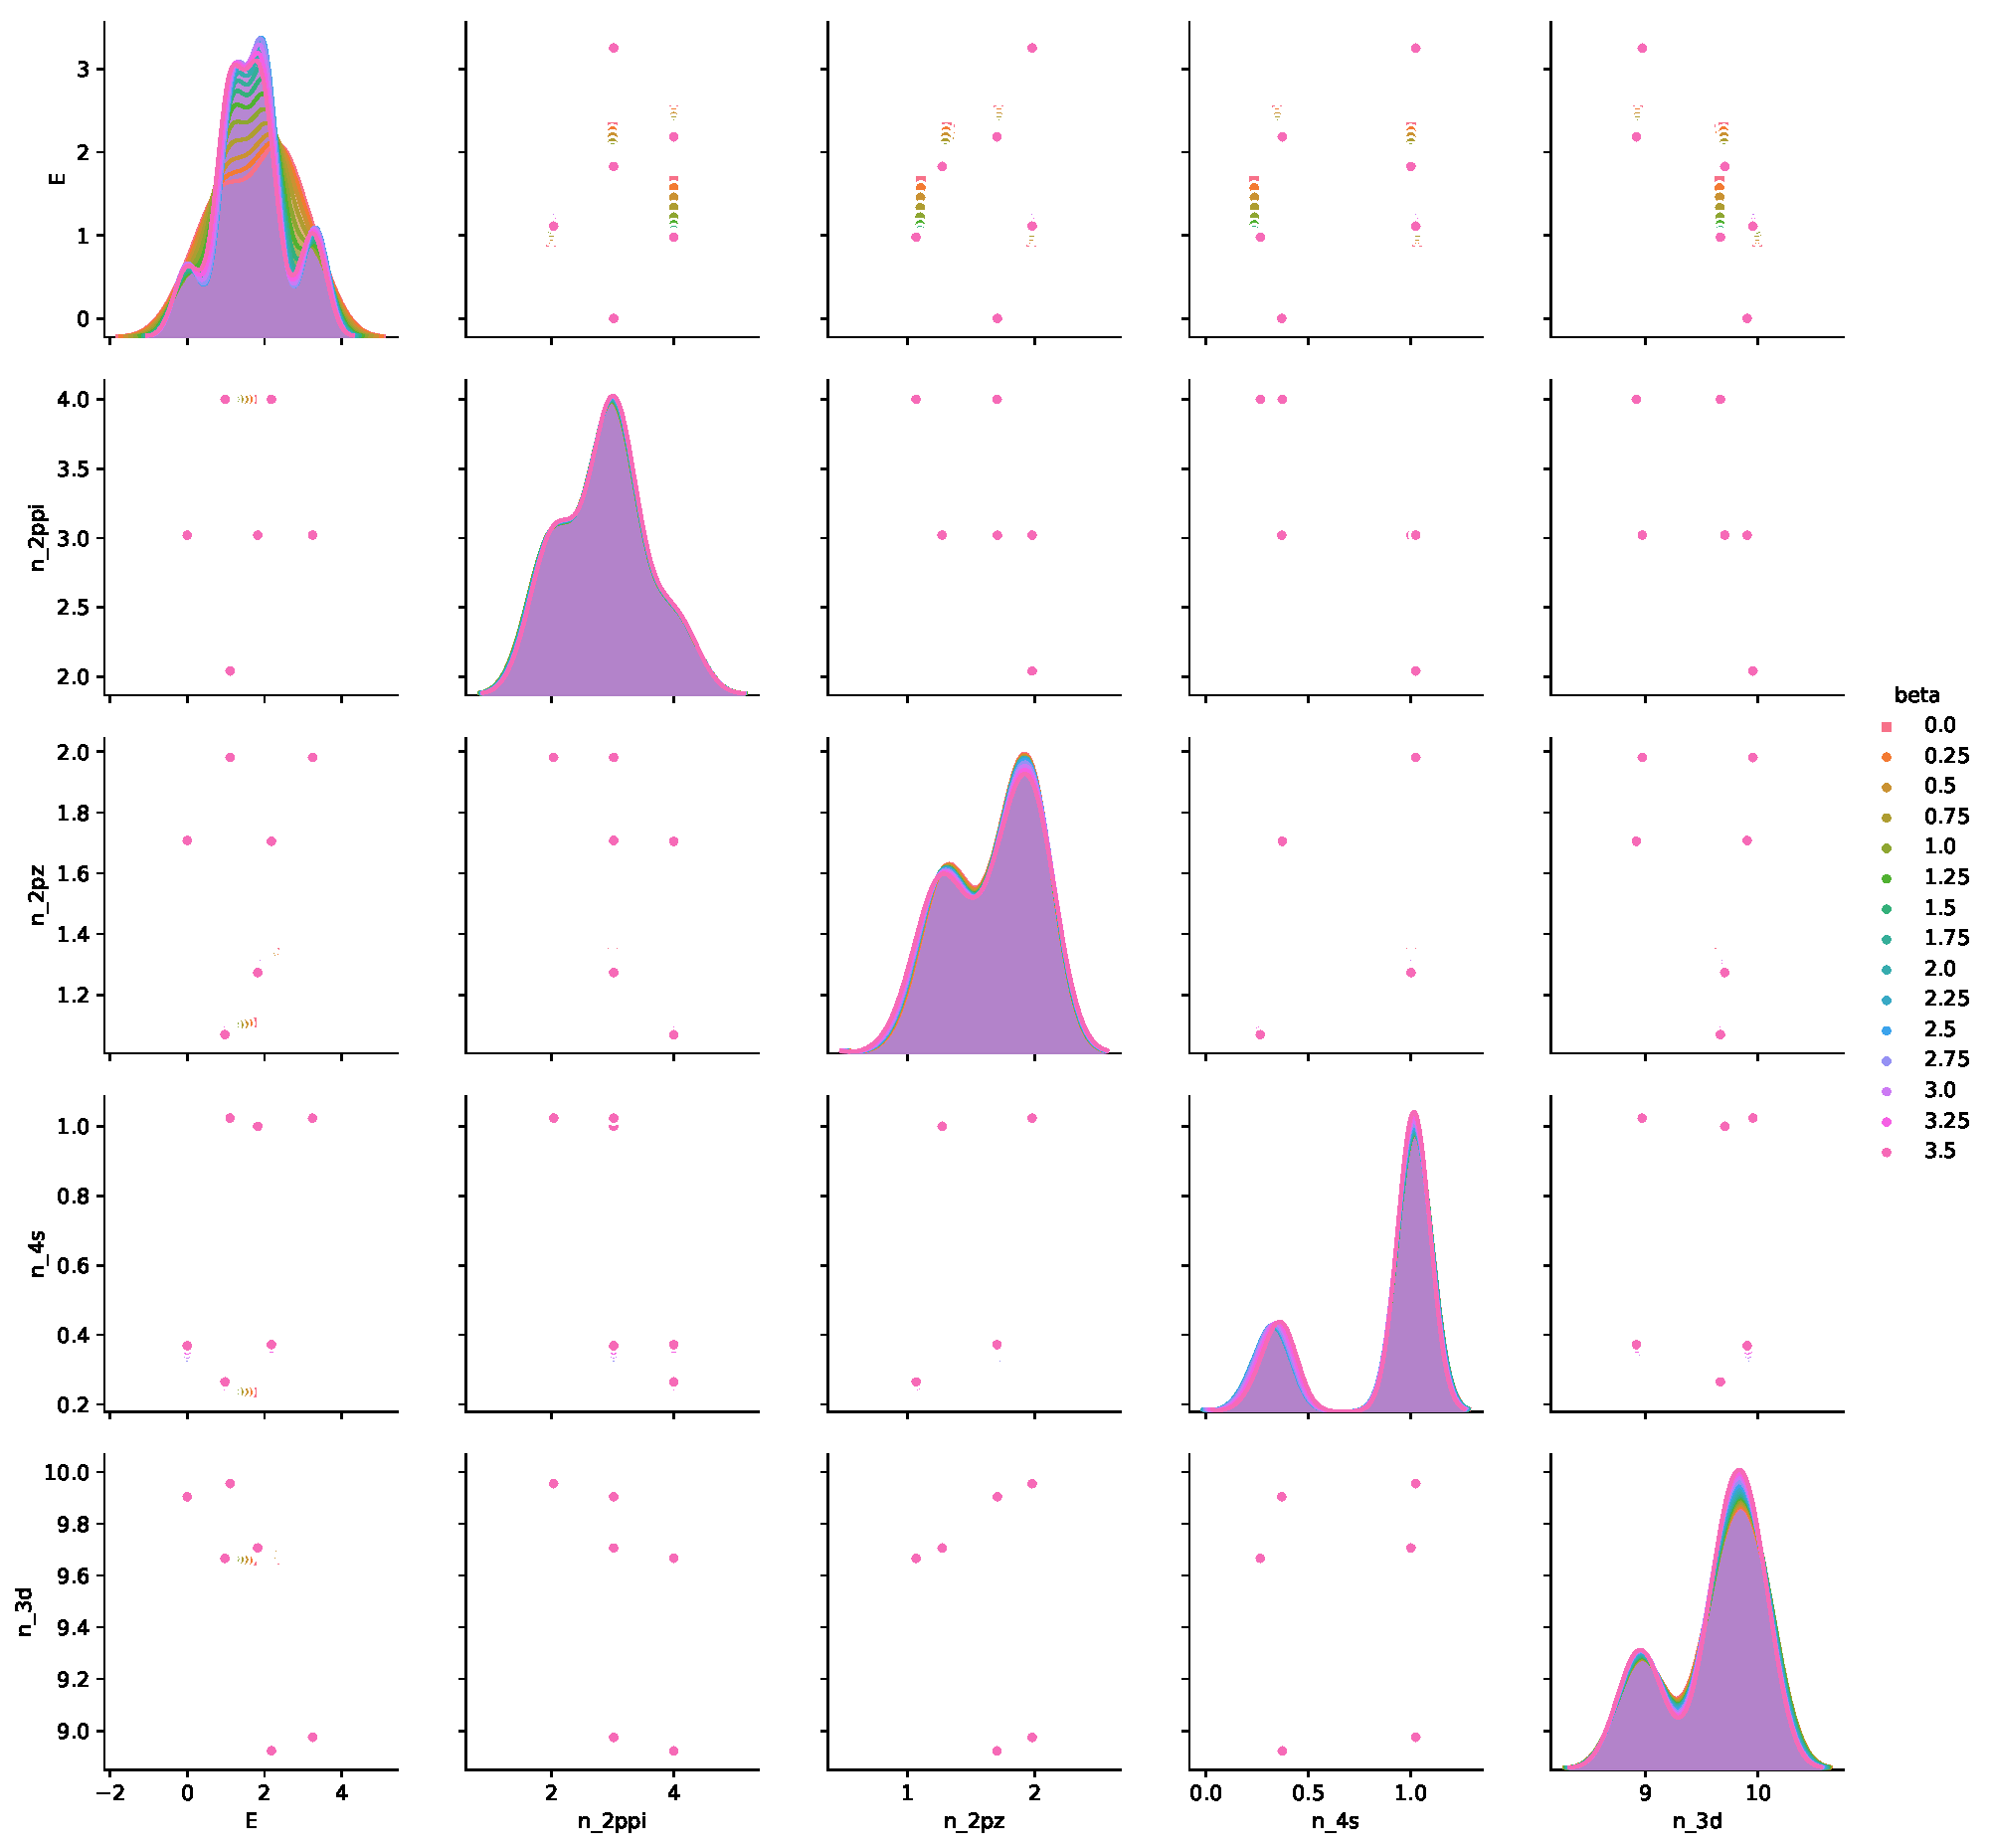
\includegraphics[width=\linewidth]{../qwalk/ub3lyp_s1_/analysis/beta_dmc_eigenvalues.pdf}
  \caption{Eigenvalues of DMC fit model, hue $\beta$.}
  \label{fig:sub1}
\end{subfigure}%
\begin{subfigure}{.5\textwidth}
  \centering
  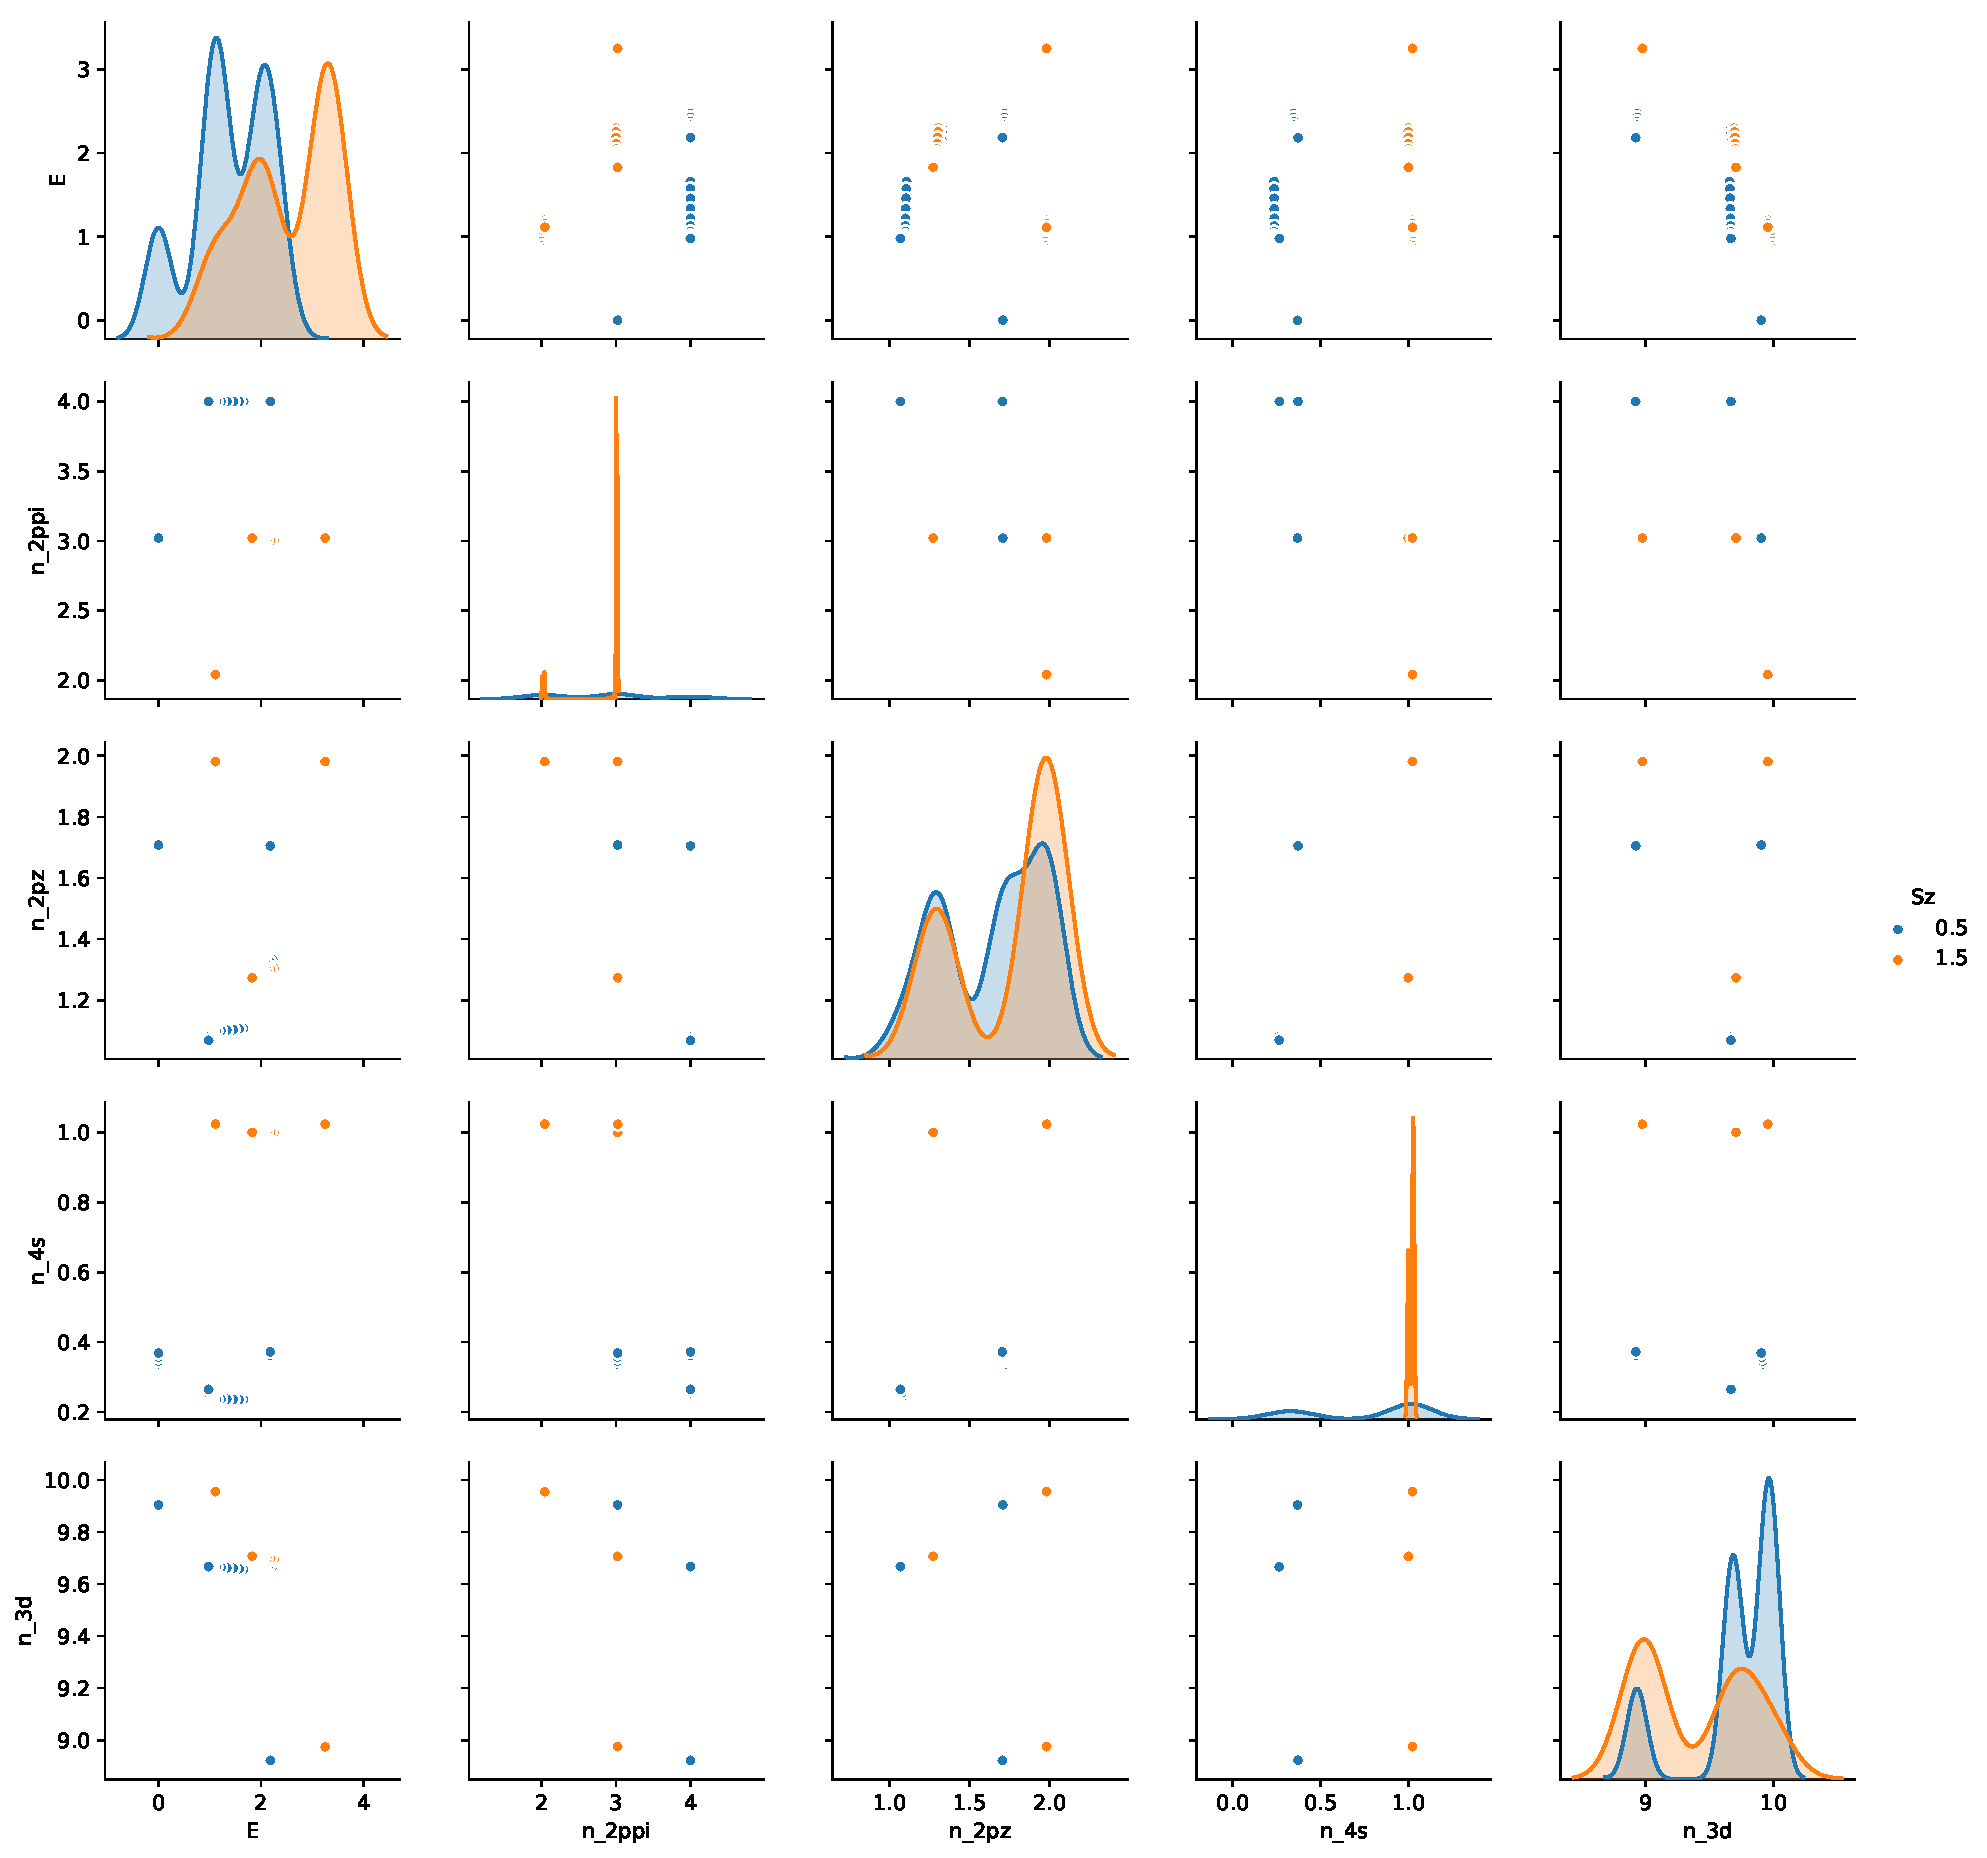
\includegraphics[width=\linewidth]{../qwalk/ub3lyp_s1_/analysis/beta_dmc_eigenvalues_sz.pdf}
  \caption{Eigenvalues of DMC fit model, hue $S_z$.}
  \label{fig:sub2}
\end{subfigure}
\label{fig:test1}
\caption{Eigenstates of models from DMC}
\end{figure}

We can compare these results to those found from, for example, an ROKS or UKS calculation of the ground state for CuO (one of our base states!). Typically one would take the ROKS/UKS eigenvalues and claim that these eigenvalues can be used as an approximate non-interacting model of the system. If we do so and exactly diagonalize in the $S_z=1/2,3/2$ sectors the ROKS/UKS eigenvalue matrix, we will find the following results for the eigenstates. The UKS eigenstates here are twice in number to the ROKS, since the UKS gives us two independent, approximate models, one for each spin channel. In table 1 below we also present the model parameters for the $\beta=2$ DMC regression compared to the ROKS model, which we will be focusing on from now on. Studying just the ROKS model for now, we see that it does predict an eigenstate at 1 eV which resembles the $^2Y$ state, however there are no low energy $S_z=3/2$ states at all. All of the $S_z=3/2$ states are $>$ 3eV above the ground state. We believe this should is due to the lack of relaxation effects present in the 1-particle model. The excited states of the CuO molecule do not look like simple 1-particle excitations on the ground state, there are relaxations of orbitals within a given symmetry sector. Further, the exclusion of the $J_{sd}$ pushes the $S_z=3/2$ states higher in energy. Clearly we see a large difference between the DMC and ROKS models, and that the DMC model more accurately reflects experiment. 

\begin{figure}
\centering
\begin{subfigure}{.5\textwidth}
  \centering
  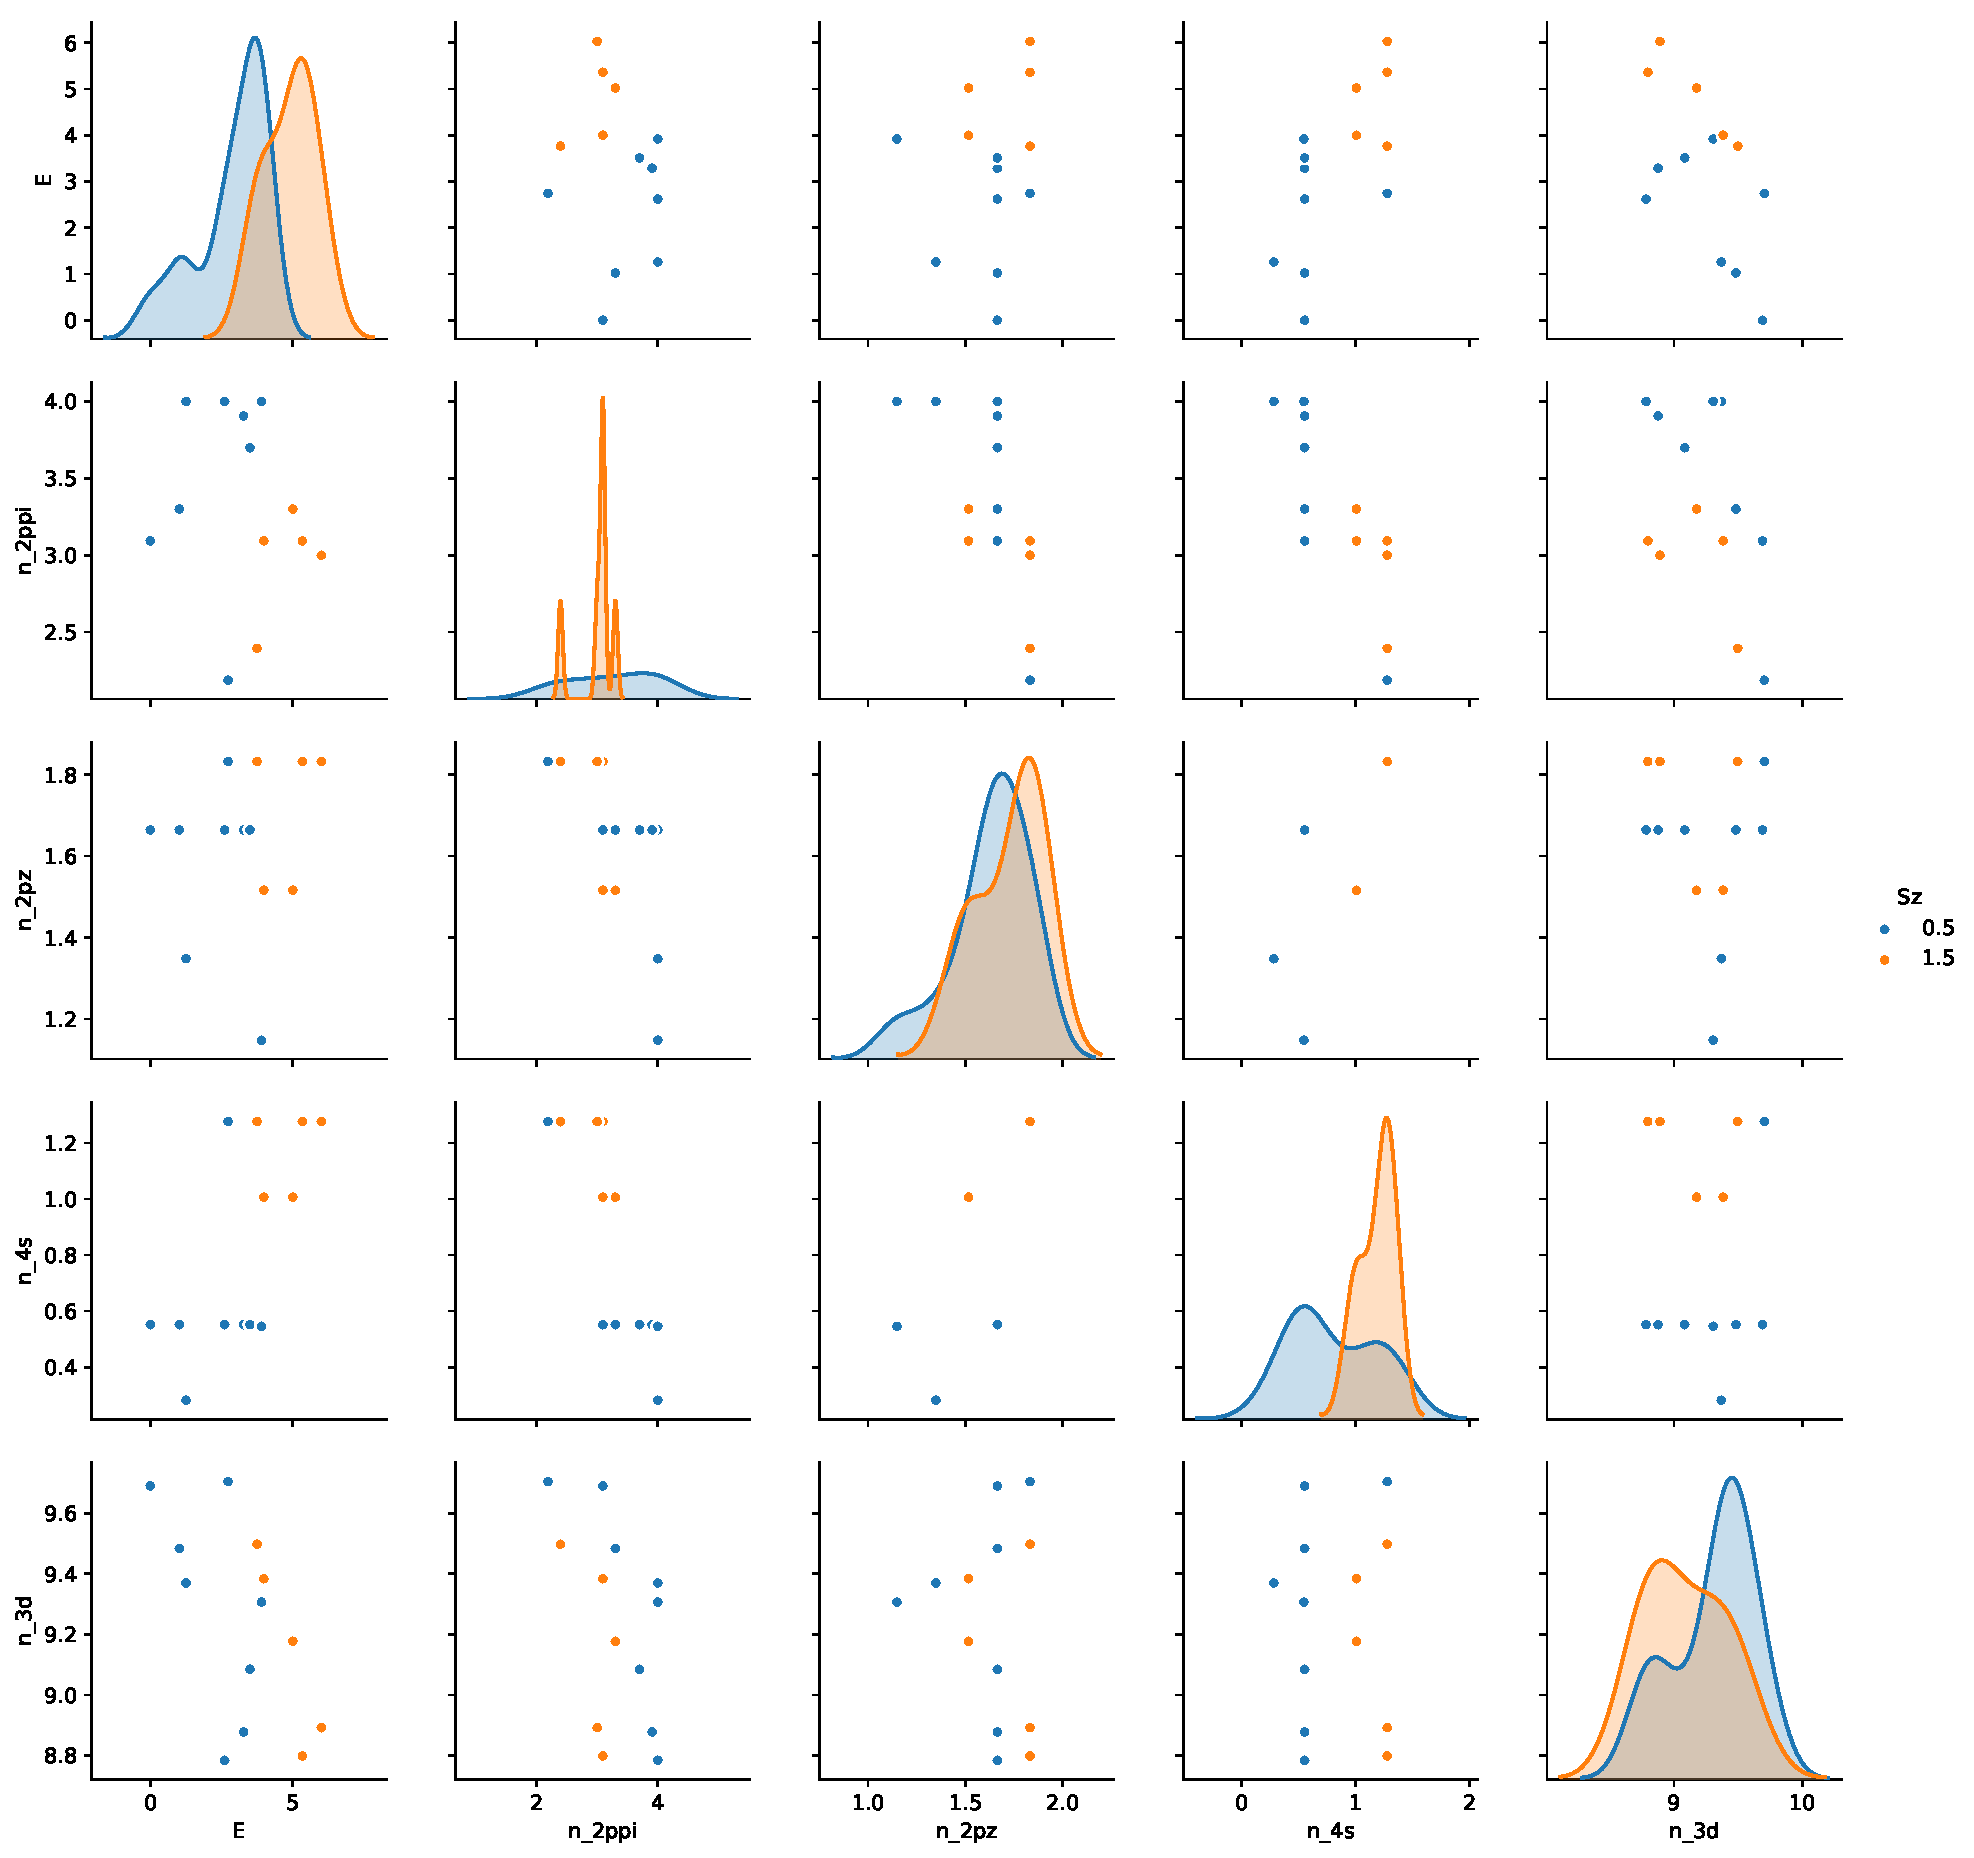
\includegraphics[width=\linewidth]{../qwalk/ub3lyp_s1_/analysis/roks_eigenvalues.pdf}
  \caption{Eigenvalues of ROKS effective model.}
  \label{fig:sub3}
\end{subfigure}%
\begin{subfigure}{.5\textwidth}
  \centering
  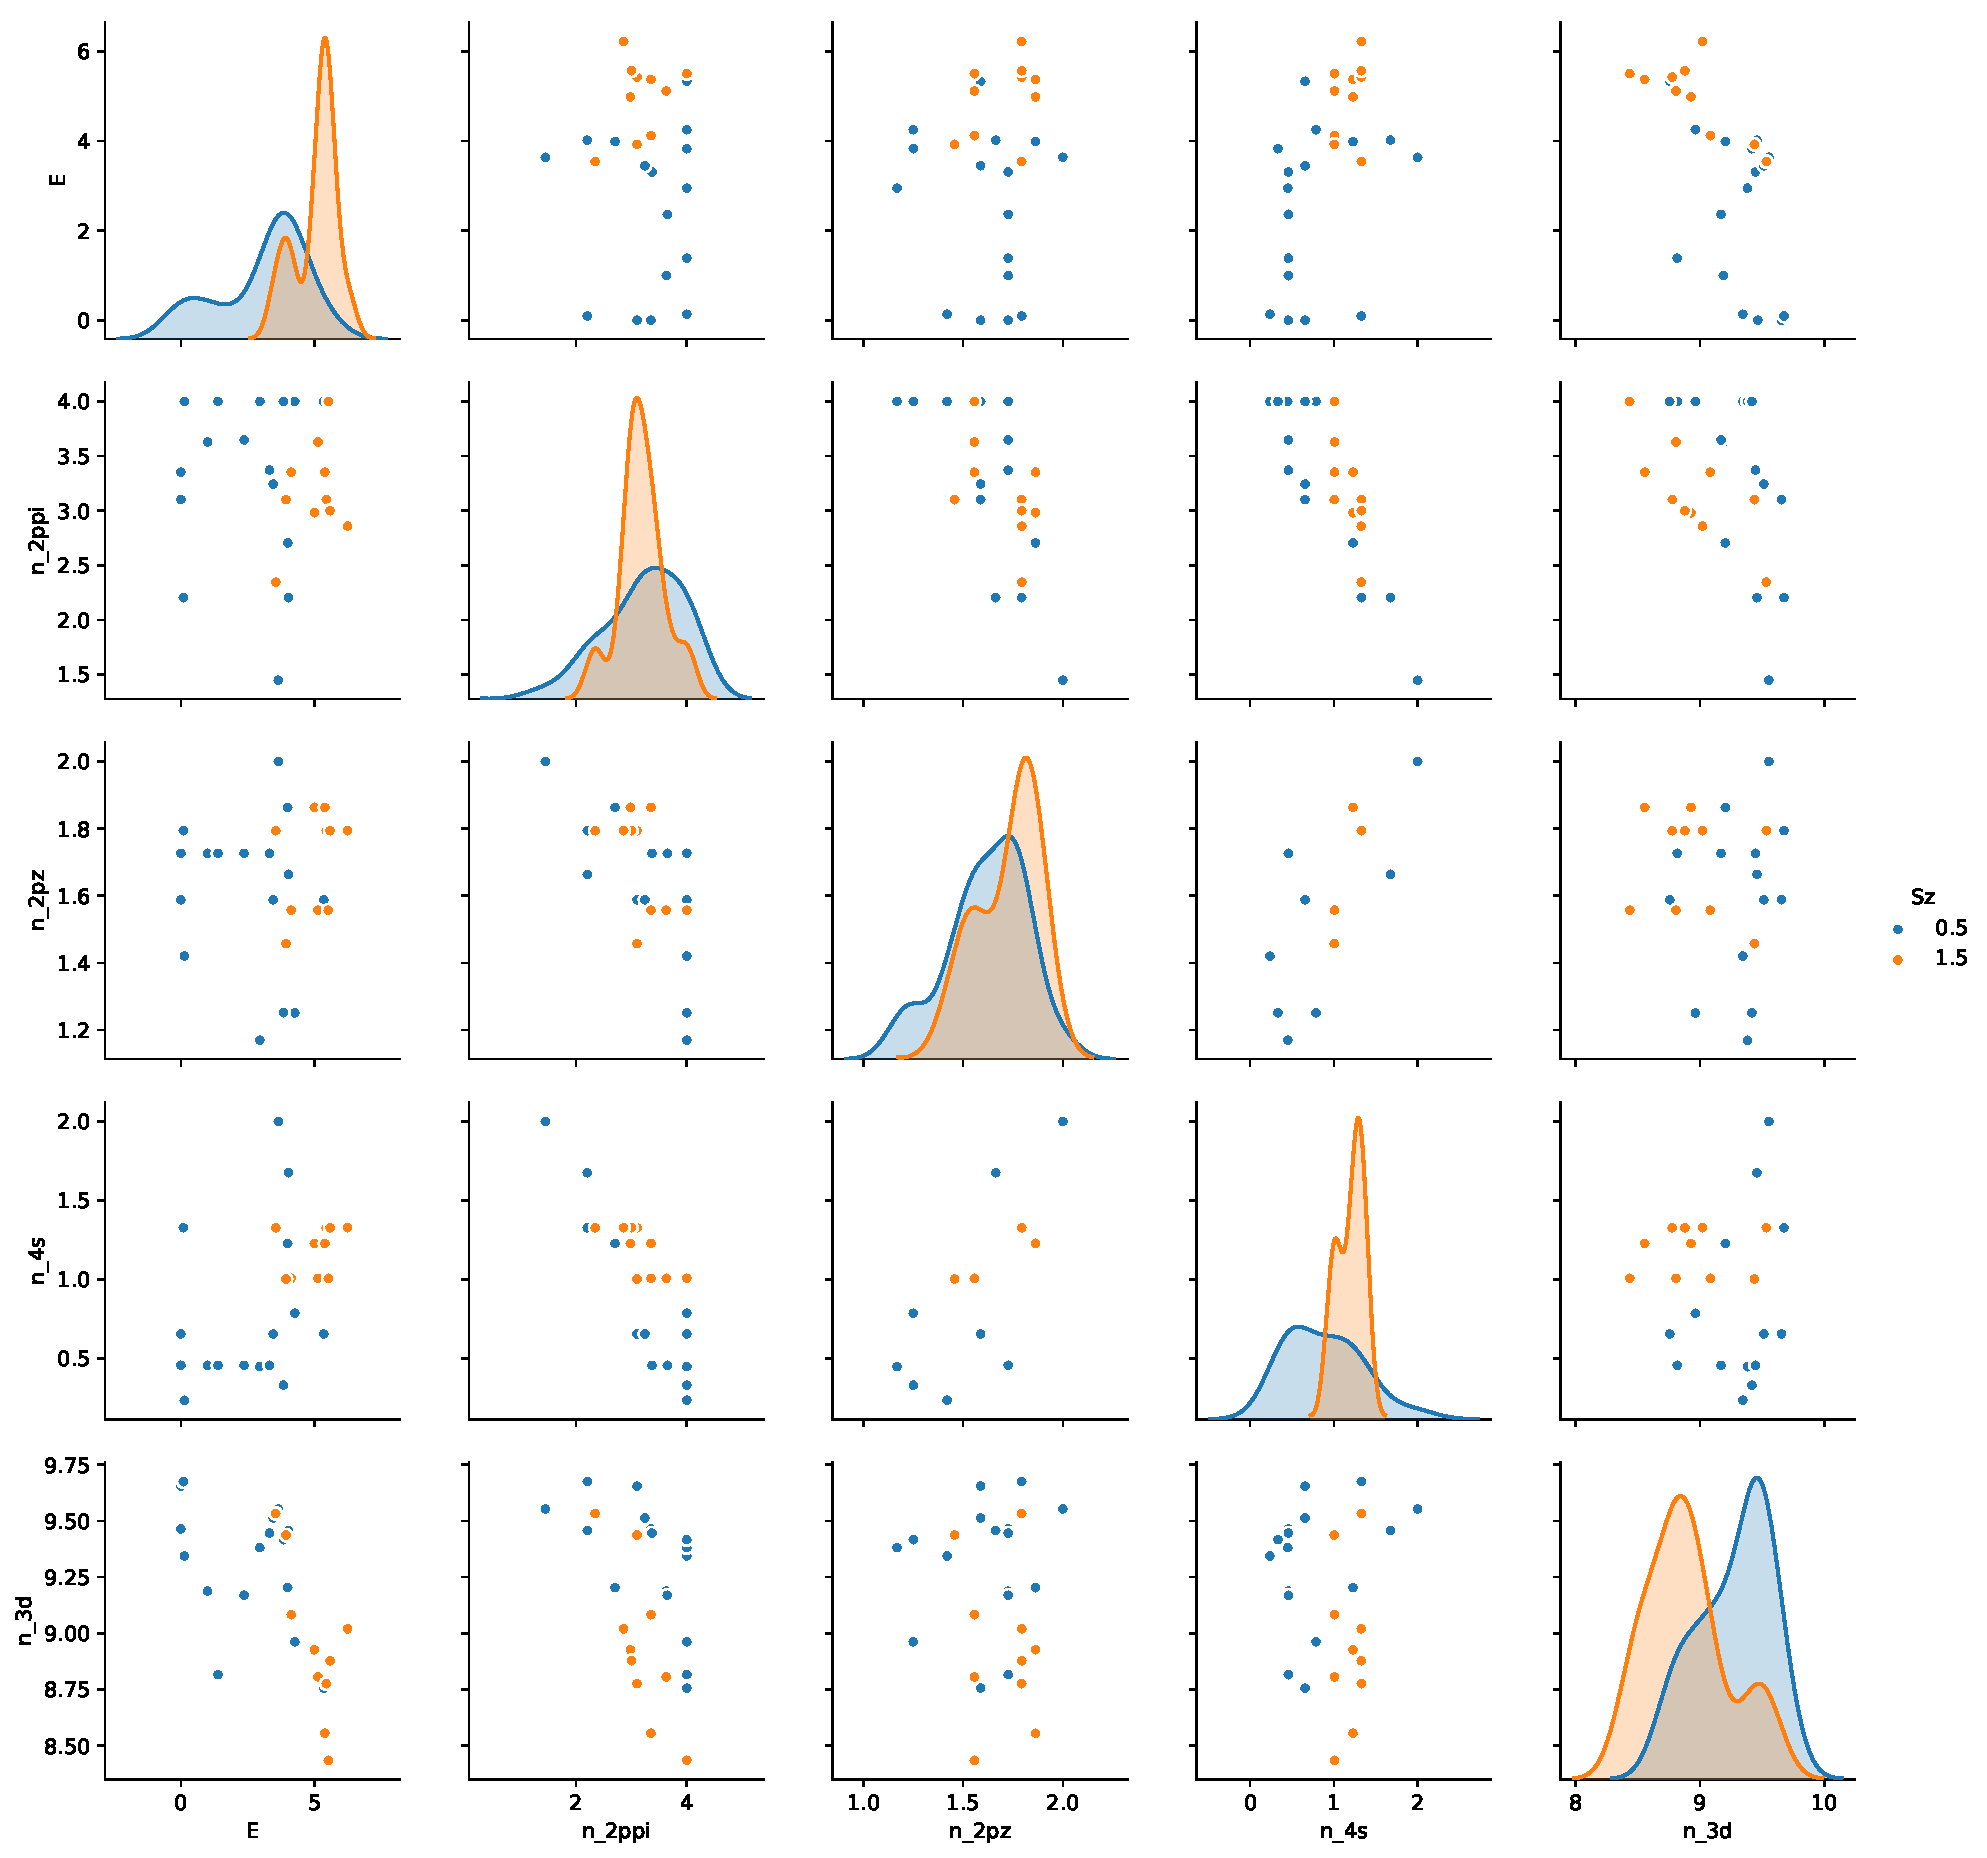
\includegraphics[width=\linewidth]{../qwalk/ub3lyp_s1_/analysis/uks_eigenvalues.pdf}
  \caption{Eigenvalues of UKS effective model.}
  \label{fig:sub4}
\end{subfigure}
\label{fig:test2}
\caption{Eigenstates of 1-particle models from DFT}
\end{figure}

\begin{wrapfigure}{r}{0.4\textwidth}
\begin{tabular}{lll}
 &  DMC (eV) & ROKS (eV) \\
$\epsilon_{d_\delta}$ &  0.00 & 0.00  \\
$\epsilon_{d_\pi}$ & -0.10 & -0.36 \\
$\epsilon_{d_{z^2}}$ & 0.41 & 0.52 \\
$\epsilon_z$ & 1.20 & 0.66 \\
$\epsilon_\pi$ & 2.21 & 0.85 \\
$\epsilon_s$ &  2.44 & 4.24 \\
$t_\pi$ & -0.22 & -1.14 \\
$t_{s d_{z^2}}$ & 0.38 & 0.97 \\
$t_{s z}$ & 0.80 & 1.86\\
$t_{d_{z^2} z}$ & 0.70 & 1.55\\
$J_{sd}$ & -0.51 & 0.00 \\ 
$U_s$ & 3.91 & 0.00 \\
\end{tabular}
\caption{Parameter differences between DFT/DMC models}
\end{wrapfigure}

\end{document}